\documentclass{standalone}
\usepackage{tikz}
\usepackage{tkz-euclide}
\usepackage{ctex}
\setCJKmainfont{Noto Serif CJK SC}
\usepackage{mhchem,siunitx}
\begin{document}
\small
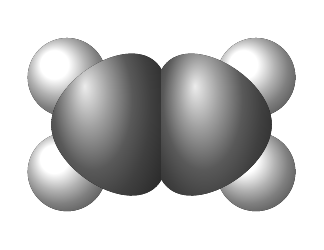
\begin{tikzpicture}[scale=1.0]

  \fill[ball color=white](-1.2,0.6)circle(0.5);
  \fill[ball color=white](-1.2,-0.6)circle(0.5);
  \fill[ball color=white](1.2,0.6)circle(0.5);
  \fill[ball color=white](1.2,-0.6)circle(0.5);
  \fill[ball color=gray](0,0.7)to[in=90,out=120](-1.4,0)to[out=-90,in=-120](0,-0.7);
  \fill[ball color=gray](0,0.7)to[in=90,out=60](1.4,0)to[out=-90,in=-60](0,-0.7);
\end{tikzpicture}
\end{document}